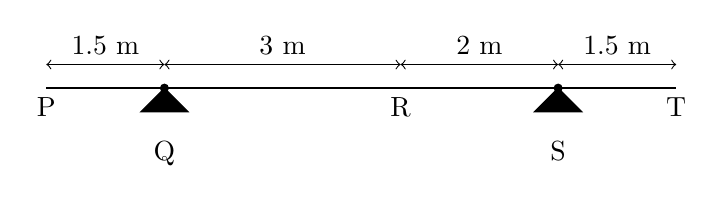
\begin{tikzpicture}

    % Draw the line
    \draw[thick] (0,0) -- (8,0);

    % Define the points along the line
    \node[below] at (0,0) {P};
    \node[below] at (1.5,-0.55) {Q};
    \node[below] at (4.5,0) {R};
    \node[below] at (6.5,-0.55) {S};
    \node[below] at (8,0) {T};

    % Add hinges at Q and S
    \draw[fill] (1.5,0) circle [radius=0.05];
    \draw[fill] (6.5,0) circle [radius=0.05];

    % Draw distances and labels
    \draw[<->] (0,0.3) -- (1.5,0.3) node[midway, above] {1.5 m};
    \draw[<->] (1.5,0.3) -- (4.5,0.3) node[midway, above] {3 m};
    \draw[<->] (4.5,0.3) -- (6.5,0.3) node[midway, above] {2 m};
    \draw[<->] (6.5,0.3) -- (8,0.3) node[midway, above] {1.5 m};

    % Draw hinge at Q
    \draw[fill=black] (1.5,0) -- (1.2,-0.3) -- (1.8,-0.3) -- cycle; % Triangle
   
    % Draw hinge at S
    \draw[fill=black] (6.5,0) -- (6.2,-0.3) -- (6.8,-0.3) -- cycle; % Triangle
  


\end{tikzpicture}
